\section{Entwurf}
\label{sec:TestEntwurf}

\begin{figure}[H]
\centering
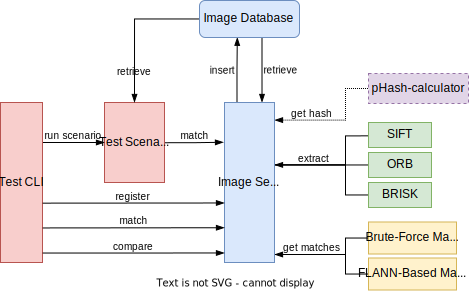
\includegraphics[scale=.3]{Abbildungen/entwurf.drawio}
\caption{Skizze Entwurf}
\label{fig:pixelkreis}
\end{figure}

Mit dem Test-System soll es m�glich sein Schl�sselpunkte und Deskriptoren aus Bildern zu extrahieren und Matches mit anderen Bildern zu finden. 
Zum extrahieren der Schl�sselpunkte und Deskriptoren kommen SIFT, ORB und BRISK (siehe Abschnitt \ref{sec:m-based}) zum Einsatz.
F�r das finden von Matches werden der Brute-Force Matcher und der FLANN-Based Matcher (siehe Abschnitt \ref{sec:MatchingStrategien}) verwendet.

Bei dem Vergleich von Bildern soll es  die M�glichkeit geben auszuw�hlen, welcher feature-based Algorithmus und welcher Matcher verwendet wird. 
Dadurch k�nnen die verschiedenen Algorithmen einzeln getestet werden.
Die gefundenen Matches werden anschlie�end mit dem "ratio test"\ (siehe Abschnitt \ref{sec:RatioTest}) gefiltert.
Der Grenzwert f�r den "ratio test"\ wird dabei auf 0.8 festgelegt. 

Mithilfe der Formel zur Bestimmung der Bild�hnlichkeit (siehe Abschnitt \ref{sec:Formel}) wird anhand der Matches ein �hnlichkeits-Score f�r die verglichenen Bilder errechnet.
Wie hoch der �hnlichkeits-Score sein muss, damit die verglichenen Bilder als Duplikate gelten, soll dynamisch festgelegt werden k�nnen.

Au�erdem sollen Bilder wahlweise auch mit pHash-Werten (siehe Abschnitt \ref{sec:pHash}) verglichen werden. 
Damit kann man das System auch f�r die Evaluation der pHash-Implementation, die in der Spread Group zum Einsatz kommt, verwenden. 
Die maximale Hamming-Distanz der pHash Werte, f�r die zwei Bilder als Duplikate gelten, wird auf 4 festgelegt.

Die Daten der Bilder, die f�r die Tests verwendet werden, werden in einer Datenbank gespeichert. 
Mit dem Test-System soll es m�glich sein Bilder f�r den Datenbanksatz und f�r die Suchsets der Test-Szenarien in der Datenbank zu registrieren. 
Beim registrieren eines neuen Bildes f�r den Datenbanksatz werden die Deskriptoren jeweils mit SIFT, ORB und BRISK, sowie der pHash Wert generiert und in der Datenbank gespeichert.
F�r die Bilder in den Suchs�tzen werden das Test-Szenario, sowie eine Referenz zum Originalbild aus dem Datenbanksatz, falls es sich um ein Duplikat handelt, gespeichert. 
Dadurch l�sst sich beim testen feststellen, ob das Suchbild richtig klassifiziert wurde.

Des Weiteren sollen auch vordefinierte Szenarien (siehe Abschnitt \ref{sec:TestSzenarien}) implementiert werden, die automatisiert ausgef�hrt werden.
Beim Durchlauf eines Szenarios wird der entsprechende Suchsatz geladen. 
Jedes Bild aus dem Suchsatz wird mit jedem Bild im Datenbanksatz abgeglichen. 
F�r jeden Durchlauf eines Szenarios werden die Metriken aus Abschnitt \ref{sec:TestMetriken} festgehalten. 

\section{Umsetzung}
\label{sec:TestUmsetzung}
Das Test-System wurde in Go \cite{go} mit der Version 1.21.0 umgesetzt. 
F�r die Bedienung des Systems wurde ein simples Kommandozeilen Interface erstellt.
Mit dem Interface lassen sich zwei gew�hlte Bilder miteinander oder ein einzelnes Bild mit den Bildern aus dem Datenbankset vergleichen. 
Au�erdem lassen sich �ber das Interface die automatisierten Test-Szenarien starten.

SIFT, ORB und BRIEF, sowie der Brute-Force und der FLANN-Based Matcher wurden �ber die Computer Vision Bibliothek OpenCV \cite{opencv} der Version 4.8.0 implementiert.
Da OpenCV keine Version f�r Go bereitstellt wird GoCV \cite{gocv} der Version 0.34.0 genutzt. GoCV bietet ein Interface f�r die C-Implemtierung von OpenCV, dass in Go nutzbar ist. F�r das persistieren der Daten der Suchsatz-Bilder und der Datenbank-Satzbilder wurde eine MySQL-Datenbank \cite{mysql} genutzt.

F�r die Einsch�tzung der Laufzeit wird die Zeit die ein Algorithmus braucht, um Schl�sselpunkte und Deskriptoren zu extrahieren, gestoppt. 
Au�erdem wird auch die Zeit gemessen, die f�r das Vergleichen der Suchbild-Deskriptoren mit den Deskriptoren der Bilder aus dem Datenbanksatz n�tig ist. 
F�r den Vergleich werden die Deskriptoren der Datenbanksatz-Bilder in Chunks aus der Datenbank geladen. 
Um zu vermeiden das die Abfragelatenz die Laufzeitmessung beeinflusst, wird f�r jedes Datenbanksatz-Bild einzeln gemessen, wie lange der Vergleich dauert.

F�r die Auswertung des Baseline-Algorithmus wird der pHash-calculator der Spread Group lokal laufen gelassen. 
Der pHash-calculator bietet bereits einen HTTP-Endpunkt, mit dem der pHash-Wert f�r einzelne Bilder errechnet werden kann.
Auch hier soll eine latenzfreie Messung der Laufzeit gew�hrleistet werden. 
Dazu wurde der pHash-calculator so erweitert, dass er die Zeit zum errechnen des pHash-wert selber misst und zusammen mit dem Hash �ber den Http-Endpunkt zur�ck gibt.
